\documentclass[11pt, oneside]{article}   	% use "amsart" instead of "article" for AMSLaTeX format
\usepackage{geometry}                		% See geometry.pdf to learn the layout options. There are lots.

\geometry{letterpaper, tmargin=1cm, bmargin=1cm, lmargin=1cm, rmargin=1cm}                   		% ... or a4paper or a5paper or ... 
%\geometry{landscape}                		% Activate for for rotated page geometry
%\usepackage[parfill]{parskip}    		% Activate to begin paragraphs with an empty line rather than an indent
\usepackage{graphicx}				% Use pdf, png, jpg, or eps with pdflatex; use eps in DVI mode
								% TeX will automatically convert eps --> pdf in pdflatex		


%% language
\usepackage[utf8]{inputenc}

\usepackage{amsfonts}
\usepackage{amsmath}
\usepackage{amssymb}
\usepackage{tikz}

%% fonts
\usepackage[T1]{fontenc}
\pagenumbering{gobble}


\title{Brief Article}
\author{The Author}
%\date{}							% Activate to display a given date or no date

\begin{document}

%% change font
\fontfamily{phv}\selectfont

\begin{tikzpicture}
%
%% PICTURE
\node [] at (-2.5,0) {
\begin{tikzpicture}
\node [rectangle] () at (0,0) {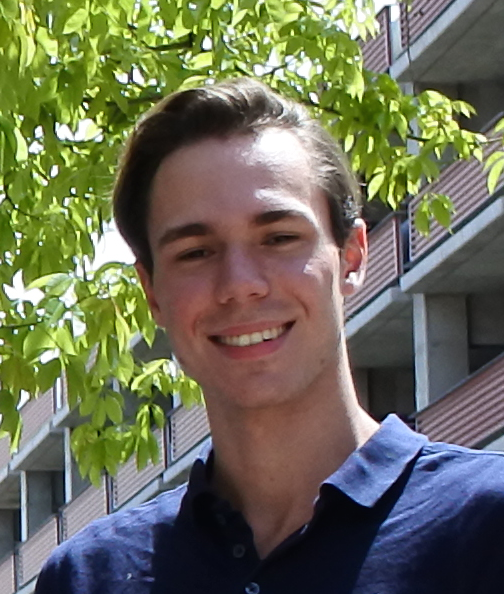
\includegraphics[width=0.15\linewidth]{figures/WILL.png}};
\end{tikzpicture}
};
%
\node [] at (5,0) {
\begin{minipage}{0.5\linewidth}
% \vspace{0.5cm}
{\LARGE \textbf{Willem Bonnaffé}} \\ 
\\
\textbf{$\mathbf{4^{th}}$ year DPhil Student (NERC DTP)} \\
61 Pusey House - St. Cross College,\\
Oxford, OX1 3LZ, UK\\
00 33 6 83 40 43 49 \\ 
willem.bonnaffe@gmail.com
\end{minipage}
};
\end{tikzpicture}

\center
\begin{tabular}{rll}
%% WORK %%
\textbf{WORK} & --------------------------------------------------------------------- &  \\
\\
2021-ongoing & \textbf{Research assistant in AI \& remote sensing} &  \textbf{University of Oxford} \\
4 months & Building ML tools to analyse forest canopy drone imagery & Department of Zoology \\
& Image processing - Image recognition - Classification & \\
\\
2020-ongoing & \textbf{Co-founder \& Lead on AI solutions} &  \textbf{Eltanin Martime Analytics} \\
12 months & AI solutions to predict weather disruptions in ports & \& Oxford University Innovation \\
& Won 2020 Oxford AI impact hackathon for climate change & \\
\\
2016-2017 & \textbf{Research assistant in Mathematical Biology} &  \textbf{University of Arizona} \\
10 months & \textit{Modelling evolution of tropical fish communities} &  Ecology and Evolutionary Biology Dpt. \\
& Bayesian modelling - MCMCMH/HMC - IBMs & \\
\\
%% EDUCATION %%
\textbf{EDUCATION} & --------------------------------------------------------------------- &  \\
\\
2017-2021 & \textbf{DPhil in AI \& Environmental Sciences} & \textbf{University of Oxford} \\
& \textit{Inferring eco-evolutionary feedbacks in nature} & NERC DTP \& Department of Zoology \\
& Expertise in AI analysis of time series data & Pr. B. Sheldon \& Pr. T. Coulson \\
\\
2020 & \textbf{Enterprise Process Labs High Intensity Training} & \textbf{University of Oxford} \\
6 months & Trained in Lean Startup Methodology for Innovation & Enterprise Process Labs \\
& Market search - Financial modelling - Prototyping & \\
\\
2013-2017 & \textbf{Diploma in Socio-Environmental Sciences} & \textbf{Ecole normale supérieure Ulm} \\
& Expertise in water and fish stock management & Environmental Research and \\
& Policy assessment - Agent-based modelling &  Teaching Institute \\
\\
2013-2016 & \textbf{MSc in Evolutionary Biology} & \textbf{Ecole normale supérieure Ulm} \\
	& $1^{st}/49$ written exams - Highest honors  & \& \textbf{Université Pierre et Marie Curie} \\
 & Advanced training in stat./mathematical modelling & \\
 \\
2011-2013 & \textbf{BSc in Life Sciences} & \textbf{Université Pierre et Marie Curie} \\
 & $5^{th}/505$ written exams - High honors  & \\
& General training in Chemistry, Physics, Biology & \\
\\
\end{tabular}

\hspace{-2.5cm}
\begin{tabular}{rll}
%% EXTRA-CURICULAR %%
\textbf{SKILLS} & --------------------------------------------------------------------- &  \\
\\
\textbf{I.T.} & Vim - \LaTeX~ - Beamer - Word - Excel - Powerpoint & \\
% \\
\textbf{Programming} & R - C/C++ - Bash - Python - NetLogo - MatLab - Julia - Mathematica & \\
% \\
\textbf{Machine learning} & Classification - Time series - Regression - NODEs - ResNets - RNNs & \\
% \\
\textbf{Languages} & French/English - German (basics) - Dutch (basics) & \\
% \\ 
\textbf{Skills} & Jazz guitar, performance, composition - Impressionist soft pastel painting - Fly fishing
\end{tabular}



%%
% \newpage
% \begin{minipage}{\linewidth}\vspace{2cm}\end{minipage}

\begin{tabular}{rll}
%% EXPERIENCE %%
\textbf{EXPERIENCE} & --------------------------------------------------------------------- &  \\
\\
2016 & \textbf{Internship in System Biology} &  \textbf{Université Pierre et Marie Curie} \\
5 months & \textit{Trophic network topology along thermal gradients} & Institute of Ecology and  \\
& Network theory - statistical modelling - bib. review & Environmental Sciences \\
\\
2015 & \textbf{Internship in Computational Biology} &  \textbf{Ecole normale sup\'erieure Ulm} \\
4 months & \textit{Fisheries and trout meta-population dynamics} & Environmental Research and  \\
& Agent-based models $C_{++}$ - numerical simulations & Teaching Institute\\
\\
2014-2015 & \textbf{Internship in Functional Ecology} &  \textbf{Université Pierre et Marie Curie} \\
6 months & \textit{Ontogeny of body colouration in lizards} & Institute of Ecology and  \\
& Spectrophotmetry - statistical modelling & Environmental Sciences \\
\\
2014 & \textbf{Internship in Behavioural Ecology} &  \textbf{University of Oxford} \\
5 months & \textit{Fitness consequences of sociality} & Department of Zoology \\
& Fieldwork - statistical modelling - network theory & \\
\\
2013 & \textbf{Internship in Cognitive Ethology} &  \textbf{Mus\'eum national d'histoire naturelle} \\
2 months & \textit{Detection of prosocial behaviour in rodents} & Laboratoire d'Ethologie Cognitive et \\
& Supervision of experiments - animal care & Compar\'ee \\
\\
%% TEACHING %%
\textbf{TEACHING} & --------------------------------------------------------------------- &  \\
\\
2020 & \textbf{Demonstrator in doctoral course} & \textbf{University of Oxford} \\
2 weeks & Machine learning modules & Doctoral Training Center \\
\\
2019-2020 & \textbf{Tutor and demonstrator in undergrad. course} & \textbf{University of Oxford} \\
6 months & Quantitative methods (2nd year BSc in Biology) & Dpt. of Zoology \\
\\
2018 & \textbf{Demonstrator in doctoral course} & \textbf{University of Oxford} \\
6 weeks & Quantitative and computational methods & NERC DTP \\
\\
%% OUTREACH %%
\textbf{CONFERENCES} & --------------------------------------------------------------------- &  \\
\\
2020 & \textbf{Festival of Ecology} & \textbf{British Ecological Society} \\
Dec. & Speaker (\textit{Eco-evo feedbacks in Darwin's finches}) & London \\
\\
2020 & \textbf{Evol. Demogr. Society's 7th annual meeting} & \textbf{Norwegian University of Sc. and Tech.} \\
Oct. & Invited speaker (\textit{AI applied to Evol. dynamics}) & Centre for Biodiversity Dynamics \\
\\
2018 & \textbf{NERC grand challenges seminar series} & \textbf{University of Oxford} \\
Dec. & Co-organized conference on Science and Politics & NERC DTP \& Jesus College\\
\\
2017 & \textbf{Trophic network research showcase 2} & \textbf{Université Pierre et Marie Curie} \\
June & Speaker (\textit{Trophic networks and thermal gradients}) & Institute of Ecology and Environmental Sc. \\
 \\
2017 & \textbf{Uncertainity Quantification showcase} & \textbf{University of Arizona} \\
April & Speaker (\textit{Bayesian analysis of ecological data}) & Department of Mathematics \\
\\
2016 & \textbf{Trophic network research showcase 1} & \textbf{Université Lille 1} \\
June & Speaker (\textit{Trophic networks and thermal gradients}) &Ecology, Evolution, and Palaeontology Unit \\
\\
% %% OUTREACH %%
% \\
% \textbf{TALKS} & --------------------------------------------------------------------- &  \\
% \\
% 2019-2020 & \textbf{Neural Differential Equations for Biology} & \textbf{University of Oxford} \\
% Nov. 2020 & Data science seminar  & Doctoral Training Center \\
% Nov. 2020 & Presentation in the Coulson Lab. group  & Dpt. of Zoology \\
% Oct. 2020 & Presentation in the Sheldon Lab. group  & \\
% Dec. 2019 & Presentation in the Coulson Lab. group  & \\
% \\
% 2019 & \textbf{Inferring evolution from time series data} & \textbf{University of Oxford} \\
% April & Presentation in the Sheldon Lab. group  & Dpt. of Zoology \\
% Febr. & Presentation in the Coulson Lab. group  & \\
% \\
% 2017 & \textbf{Bayesian modelling workshop} & \textbf{University of Arizona} \\
% April & Demonstrated Bayesian analysis of ecological data & Tree ring Lab. \\
% \\
\end{tabular}

\begin{tabular}{rll}
%% PUBLICATIONS %%
\\
\textbf{PUBLICATIONS} & --------------------------------------------------------------------- & \\
\\
2021 & \textit{Inferring eco-evolutionary feedbacks} & In prep. \\ 
& \textit{from time series data} & \\
& W. Bonnaff\'e, B.C. Sheldon \& T. Coulson & \\
\\
2021 & \textit{Uncovering Eco-evo feedbacks in Darwin's Finches} & In prep. \\ 
& \textit{with Neural Ordinary Differential Equations} & \\
& W. Bonnaff\'e, B.C. Sheldon \& T. Coulson & \\
\\
2021 & \textit{Inconsistent species interaction in replicated systems} & Submitted to Ecology Letters \\ 
& \textit{may hinder generalisation of dynamical processes} & \\
& W. Bonnaff\'e \& T. Coulson & \\
\\
2021 & \textit{Species richness and network structure  } & Submitted to Ecology Letters \\ 
& \textit{jointly drive total biomass and its} & \\
& \textit{temporal stability in fish communities} & \\
& A. Danet, E.Thebault,  W. Bonnaff\'e,  M. Mouchet \& O. Collin &\\
\\
2021 & \textit{Neural Ordinary Differential Equations for} & Methods in Ecology  \\ 
& \textit{Ecological and Evolutionary time series analysis} & and Evolution \\
& W. Bonnaff\'e, B.C. Sheldon \& T. Coulson & \\
\\
2021 & \textit{Comparison of size-structured and species-level trophic} & Oikos \\ 
& \textit{networks reveals antagonistic effects of temperature on} & \\
& \textit{species-level response to temperature} & \\
& W. Bonnaff\'e, S. Legendre, A. Danet, \& E. Edeline & \\
\\
2018 & \textit{Ontogenetic trajectories of body colouration} & Ecology and Evolution \\ 
& \textit{reveal its function as a multicomponent} & \\
& \textit{non-senescent signal} &  \\
& W. Bonnaff\'e et al. \\
\\
\end{tabular}

\end{document}  
